
\documentclass[10pt,twocolumn,letterpaper,sort&compress]{article}

\usepackage{iccv}
\usepackage{times}
\usepackage{epsfig}
\usepackage{graphicx}
\usepackage{amsmath}
\usepackage{amssymb}
\usepackage[numbers,sort]{natbib}

\usepackage{subfigure}
\usepackage{upgreek}
\usepackage{multirow}
\usepackage{color}
\usepackage{bm}
\DeclareMathOperator*{\argmin}{arg\,min}
\usepackage{arydshln}
\usepackage{latexsym}

\usepackage{amsthm}
\newtheorem{theorem}{Theorem}
\newtheorem{lemma}[theorem]{Lemma}
\newtheorem{conj}[theorem]{Conjecture}


% Include other packages here, before hyperref.

% If you comment hyperref and then uncomment it, you should delete
% egpaper.aux before re-running latex.  (Or just hit 'q' on the first latex
% run, let it finish, and you should be clear).
\usepackage[pagebackref=true,breaklinks=true,letterpaper=true,colorlinks,bookmarks=false]{hyperref}
\renewcommand{\huge}{\fontsize{8pt}{\baselineskip}\selectfont}

% \iccvfinalcopy % *** Uncomment this line for the final submission

\def\iccvPaperID{572} % *** Enter the ICCV Paper ID here
\def\httilde{\mbox{\tt\raisebox{-.5ex}{\symbol{126}}}}

% Pages are numbered in submission mode, and unnumbered in camera-ready
\ificcvfinal\pagestyle{empty}\fi
\begin{document}

%%%%%%%%% TITLE
\title{Multi-channel Weighted Nuclear Norm Minimization for Real Color Image Denoising}

\author{First Author\\
Institution1\\
Institution1 address\\
{\tt\small firstauthor@i1.org}
% For a paper whose authors are all at the same institution,
% omit the following lines up until the closing ``}''.
% Additional authors and addresses can be added with ``\and'',
% just like the second author.
% To save space, use either the email address or home page, not both
\and
Second Author\\
Institution2\\
First line of institution2 address\\
{\tt\small secondauthor@i2.org}
}

\maketitle
%\thispagestyle{empty}

%%%%%%%%% ABSTRACT
\begin{abstract}
The noise structures among the R, G, B channels of real images are quite different due to the preprocessing steps, such as demosaicing, white balance, etc., of the in-camera imaging pipelines. This makes the real image denoising problem much more complex than tranditional grayscale image denoising. In this paper, we propose a multi-channel optimization model for real color image denoising.\ Specifically, we introduce a weighting matrix into the data term to process adaptively each part of R, G, B channels in the joint patches concatenated by corresponding patches in these channels.\ In the regularization term, we employ the weighted nuclear norm to exploit the non-local self similar property.\ The proposed multi-channel weighted nuclear norm minimization (WNNM) model is much more complex than the standard WNNM model.\ We reformulate the proposed model into a linear constrained optimization problem and solve it by the alternating direction method of multipliers algorithm.\ Each alternative updating step has closed-form solution and the convergence results are given.\ Experiments on benchmark datasets demonstrate that the proposed model outperforms state-of-the-art denoising methods on synthetic as well as real-world noisy images.
\end{abstract}

\section{Introduction}


Image denoising is an important problem in enhancing the image quality in computer vision systems. The traditional grayscale image denoising problem aims to recover the clean image $\mathbf{x}$ from the noisy observation $\mathbf{y}=\mathbf{x}+\mathbf{n}$, where $\mathbf{n}$ is often assumed to be additive white Gaussian noise (AWGN). Most image denoising methods in this field either employ the non-local self similarity (NSS) of natural images \cite{nlm,bm3d,ksvd,lssc,ncsr,pgpd,wnnm} or learn generative or discriminative denoisers from paired natural clean images and synthetic noisy images \cite{foe,epll,mlp,csf,chen2015learning}. Among these methods, the weighted nuclear norm minimization (WNNM) method achieves excallent denoising performance by exploiting the NSS property via low rank regularization. 

The real color image denoising problem is not a trivial extension from single channel (grayscale image) to multiple channels (color image). The reason is that the noise structures are quite different among the R, G, B channels of images captured by CCD or CMOS cameras due to the on-board processing steps \cite{karaimer_brown_ECCV_2016}. This makes the real color image denoising problem much more complex. Directly applying the denoising methods for grayscale images to each channel of color images seperately would obtain bad performance \cite{mairal2008sparse}. There are several work  \cite{cbm3d,mairal2008sparse,Liu2008,noiseclinic,crosschannel2016,Zhu_2016_CVPR} proposed specifically for color image denoising. The method \cite{cbm3d} first transforms the color images into the luminance/chrominance space such as YCbCr before denoising, but this would make the noise distribution more complex in color images. The methods of \cite{mairal2008sparse,Zhu_2016_CVPR} process the joint patches concatenated by the corresponding patches in R, G, B channels and treat equally the patches in different channels. This would would generate false colors or artifacts \cite{mairal2008sparse}. The methods of \cite{Liu2008,noiseclinic,crosschannel2016} ignore the non-local self similarity property of natural images, and their performance would be largely depressed \cite{bm3d,wnnm}.

In order to deal with the R, G, B channels in color images more effectively, different noise properties of different channels should be considered in solving real color image denoising problem. Besides, due to its expressive denoising performance, the WNNM model \cite{wnnm} is employed to exploit the NSS property of natural images. In this paper, we proposed a multi-channel WNNM model for real color image denoising. By introducing a weighting matrix to the WNNM model, the proposed multi-channel WNNM model no longer has closed-form solutions and more challenging to solve. By reformulating the proposed multi-channel WNNM model into a linear constrained program with two variables, the relaxed problem can be solved under the alternating direction method of multipliers (ADMM) \cite{admm} framework. Each variable can be updated with closed-form solution \cite{wnnm,lugsvt}. We also give the convergency resutls with detailed proof to guarantee a rational termination of the proposed algorithm. 

\section{Related Work}

\subsection{Weighted Nuclear Norm Minimization}
As an extension to the nuclear norm minimization (NNM) model \cite{cai2010singular}, the weighted nuclear norm minimization (WNNM) model \cite{wnnm} is desribed as 
\vspace{-3mm}
\begin{equation}
\label{ea}
\vspace{-3mm}
\min_{\mathbf{X}}\|\mathbf{Y}-\mathbf{X}\|_{F}^{2}
+
\|\mathbf{X}\|_{\bm{w},*}
\end{equation}
where $\|\mathbf{X}\|_{\bm{w},*}=\sum_{i}w_{i}\sigma_{i}(\mathbf{X})$ is the weighted nuclear norm of matrix $\mathbf{X}$, and $\bm{w}=[w_{1},...,w_{n}]^{\top}, w_{i}\ge 0$ is the weight vector, $\sigma_{i}(\mathbf{X})$ is the $i$-th singular value of matrix $\mathbf{X}$.\ According to the Corollary 1 of \cite{wnnmijcv}, the problem (\ref{ea}) has closed-form solution if the weights are non-decreasing
\vspace{-3mm}  
\begin{equation}
\label{eb}
\vspace{-3mm}
\mathbf{\hat{X}}
=
\mathbf{U}
\mathcal{S}_{\bm{w}/2}
(\mathbf{\Sigma})
\mathbf{V}^{\top}
\end{equation}
where $\mathbf{Y}=\mathbf{U}\mathbf{\Sigma}\mathbf{V}^{\top}$ is the singular value decomposition \cite{eckart1936approximation} of $\mathbf{Y}$ and 
$\mathcal{S}_{\tau}(\bullet)$ is the generalized soft-thresholding operator with weight vector $\bm{w}$:
\vspace{-3mm}
\begin{equation}
\label{ec}
\vspace{-3mm}
\mathcal{S}_{\bm{w}/2}
(\mathbf{\Sigma}_{ii})
=
\max(\mathbf{\Sigma}_{ii}-w_{ii}/2, 0)
\end{equation}

Though having achieved excallent performance on grayscale image denoising, the WNNM model would generate false colors or artifacts \cite{mairal2008sparse}, if being directly extended to real color image denoising by processing each channel seperately or joint vectors concatenated by multiple channels. In this paper, for real noisy image denoising, we propose a multi-channel WNNM model which preserve the power of WNNM and be able to process the differences among different channels.

\subsection{Real Color Image Denoising}
During the last decade, several denoising methods are proposed for real color image denoising \cite{cbm3d,Liu2008,Zhu_2016_CVPR,noiseclinic}. Among them, the CBM3D \cite{cbm3d} first transform the RGB image into luminance-chrominance space (e.g., YCbCr) and then apply the famous BM3D method \cite{bm3d} on each channel separately with the patches being grouped only in the luminance channel. In \cite{Liu2008}, the authors proposed the ``Noise Level Function'' to eatimate and remove the noise for each channel in natural images. However, the methods processing each channel seperately would achieve inferior performance than processing jointly these channels \cite{mairal2008sparse}. The methods of \cite{noiseclinic,ncwebsite,Zhu_2016_CVPR} perform real color image denoising by concatenating the patches in R, G, B channels into joint vectors. However, the concatenation would treat each channel equally and ignore the different noise properties among these channels. The method in \cite{crosschannel2016} models the cross-channel noise in real noisy image as a multivariate Gaussian and the noise is removed by the Bayesian nonlocal means filter \cite{kervrann2007bayesian}. The commercial software Neat Image \cite{neatimage} estimates the noise parameters from a flat region of the given noisy image and filters the noise correspondingly. But these methods \cite{crosschannel2016,neatimage} ignore the non-local self similarity property of natural images \cite{bm3d,wnnm}. 

In this paper, we introduce a weighting matrix which add differents weights to different channels for color image denoising. The proposed multi-channel method can effectively solve the problem of different noise structures among different channels.

\section{Color Image Denoising via Multi-channel Weighted Nuclear Norm Minimization}

\subsection{The Problem}
\begin{figure*}
\vspace{1mm}
\centering
\subfigure{
\begin{minipage}[t]{0.25\textwidth}
\centering
\raisebox{-0.15cm}{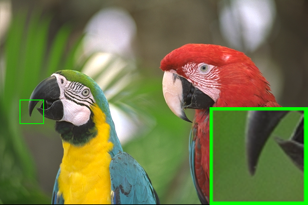
\includegraphics[width=1\textwidth]{example/resize_br_kodim23}}
{\footnotesize (a) kodim23}
\end{minipage}
\begin{minipage}[t]{0.25\textwidth}
\centering
\raisebox{-0.15cm}{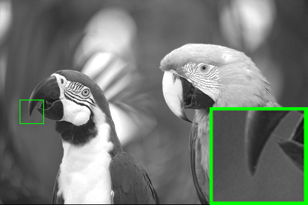
\includegraphics[width=1\textwidth]{example/resize_br_kodim23_1}}
{\footnotesize (b) kodim23: Red Channel}
\end{minipage}
\begin{minipage}[t]{0.25\textwidth}
\centering
\raisebox{-0.15cm}{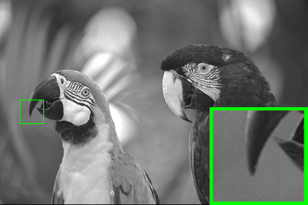
\includegraphics[width=1\textwidth]{example/resize_br_kodim23_2}}
{\footnotesize (c) kodim23: Green Channel}
\end{minipage}
\begin{minipage}[t]{0.25\textwidth}
\centering
\raisebox{-0.15cm}{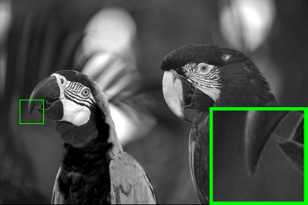
\includegraphics[width=1\textwidth]{example/resize_br_kodim23_3}}
{\footnotesize (d) kodim23: Blue Channel}
\end{minipage}
}\vspace{-4mm}
\subfigure{
\begin{minipage}[t]{0.25\textwidth}
\centering
\raisebox{-0.15cm}{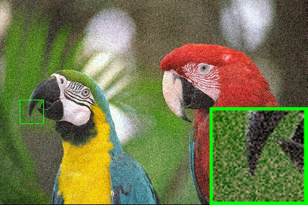
\includegraphics[width=1\textwidth]{example/resize_br_Noisy_nSig402030_kodim23.png}}
{\footnotesize (e) Noisy }
\end{minipage}
\begin{minipage}[t]{0.25\textwidth}
\centering
\raisebox{-0.15cm}{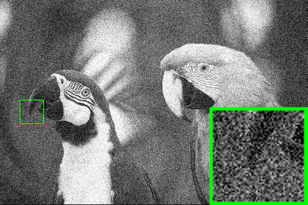
\includegraphics[width=1\textwidth]{example/resize_br_Noisy_nSig402030_kodim23_1.png}}
{\footnotesize (f) Noisy: Red Channel}
\end{minipage}
\begin{minipage}[t]{0.25\textwidth}
\centering
\raisebox{-0.15cm}{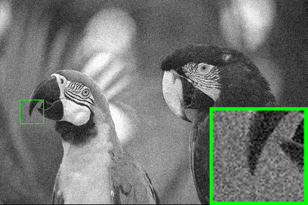
\includegraphics[width=1\textwidth]{example/resize_br_Noisy_nSig402030_kodim23_2.png}}
{\footnotesize (g) Noisy: Green Channel}
\end{minipage}
\begin{minipage}[t]{0.25\textwidth}
\centering
\raisebox{-0.15cm}{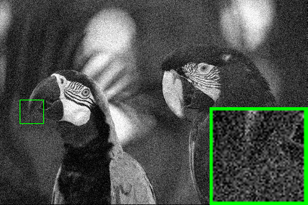
\includegraphics[width=1\textwidth]{example/resize_br_Noisy_nSig402030_kodim23_3.png}}
{\footnotesize (h) Noisy: Blue Channel}
\end{minipage}
}\vspace{-4mm}
\subfigure{
\begin{minipage}[t]{0.25\textwidth}
\centering
\raisebox{-0.15cm}{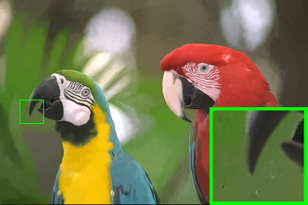
\includegraphics[width=1\textwidth]{example/resize_br_WNNM_nSig402030_lambda1_kodim23.png}}
{\footnotesize (i) WNNM}
\end{minipage}
\begin{minipage}[t]{0.25\textwidth}
\centering
\raisebox{-0.15cm}{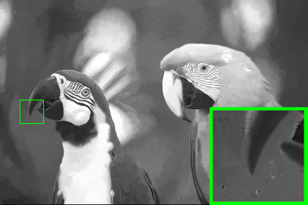
\includegraphics[width=1\textwidth]{example/resize_br_WNNM_nSig402030_lambda1_kodim23_1.png}}
{\footnotesize (j) WNNM: Red Channel}
\end{minipage}
\begin{minipage}[t]{0.25\textwidth}
\centering
\raisebox{-0.15cm}{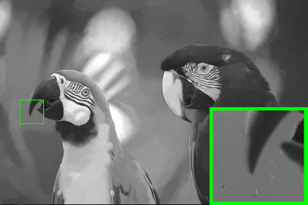
\includegraphics[width=1\textwidth]{example/resize_br_WNNM_nSig402030_lambda1_kodim23_2.png}}
{\footnotesize (k) WNNM: Green Channel}
\end{minipage}
\begin{minipage}[t]{0.25\textwidth}
\centering
\raisebox{-0.15cm}{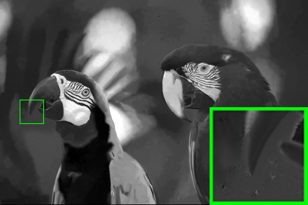
\includegraphics[width=1\textwidth]{example/resize_br_WNNM_nSig402030_lambda1_kodim23_3.png}}
{\footnotesize (l) WNNM: Blue Channel}
\end{minipage}
}\vspace{-1mm}
\caption{The image ``kodim23'' of the Kodak PhotoCD dataset, its degraded version, and the image recovered by WNNM. The R, G, B channels are also listed here for image quality comparison.}
\label{fa}
\vspace{-2mm}
\end{figure*}

The color image denoising problem can be formulated as follows: given a color image with Red (R), Green (G), Blue (B) channels, each channel is degraded by a certain of synthetic or real noise and we aim to recover the clean image from the degraded version. We argue that it is problematic to directly applying the WNNM method to the joint vectors concatenated by corresponding patches of the R, G, B channels. In Fig.\ \ref{fa}, we show the clean image of ``kodim23'' from the Kodak PhotoCD dataset, its degraded version, and the denoised image by WNNM \cite{wnnm} on the joint patches. The degraded image is generated by adding synthetic additive white Gaussian noise (AWGN) to each channel of the clean image. The standard derivations of the noise added to the R, G, B channels are $\sigma_{r}=40$, $\sigma_{g}=20$, $\sigma_{b}=30$, respectively.\ The input standard derivation of noise for the WNNM method is the Root Mean Square of those in the three channels, i.e., $\sigma=\sqrt{(\sigma_{r}^{2}+\sigma_{g}^{2}+\sigma_{b}^{2})/3}=31.1$. One can see that the WNNM method treating each channel equally would remain some noise in the R and B channel, while oversmoothing the G channel. 

In order to treat each channel differently in color image denoising, we propose to introduce a weighting matrix $\mathbf{W}$ to the original WNNM model \cite{wnnm} and the resulting multi-channel WNNM model is
\begin{equation}
\min_{\mathbf{X}}\|\mathbf{W}(\mathbf{Y}-\mathbf{X})\|_{F}^{2}
+ 
\|\mathbf{X}\|_{\bm{w},*}.
\end{equation}
where $\mathbf{W}$ is the weighting matrix. For simplisity, we assume $\mathbf{W}$ to be a diagonal matrix. Unfortunately, the proposed multi-channel WNNM problem cannot be solved in an analytical form. In \cite{wnnmijcv}, when the weights on singular values are non-descending, the weighted nuclear norm proximal operator can have global optimum with closed-form solution. However, such property is not valid for the multi-channel WNNM model. The reason is that the weighting matrix $\mathbf{W}$ is added to the matrix $\mathbf{X}$ instead of its singular values. Besides, the elements in $\mathbf{W}$ is not in a non-descending order with respect to the singular value of $\mathbf{X}$. This makes the proposed model more difficult to optimize than the original WNNM model.

This can be solved by introducing an augmented variable $\mathbf{Z}$, and the above multi-channel WNNM problem is equivalent to a linearly constrained non-convex problem with two variables.
\begin{equation}
\min_{\mathbf{X},\mathbf{Z}}\|\mathbf{W}(\mathbf{Y}-\mathbf{X})\|_{F}^{2}
+
\|\mathbf{Z}\|_{\bm{w},*}
\quad
\text{s.t.}
\quad
\mathbf{X}=\mathbf{Z}.
\end{equation}
This is an optimization problem with functions of two variables $\mathbf{X}$ and $\mathbf{Z}$ with linearly constrained condition of $\mathbf{X}=\mathbf{Z}$. In fact, this proplem can be solved by the alternating direction method of multipliers (ADMM) algorithm, which will be introduced in the next subsection.

\subsection{The Setting of Weights}
Assume the matrix $\mathbf{Y}$ containing the noisy patches in R, G, B channels as $\mathbf{Y}=[\mathbf{Y}_{r}^{\top}\ \mathbf{Y}_{g}^{\top}\ \mathbf{Y}_{b}^{\top}]^{\top}$, the corresponding clean matrix $\mathbf{X}=[\mathbf{X}_{r}^{\top}\ \mathbf{X}_{g}^{\top}\ \mathbf{X}_{b}^{\top}]^{\top}$, and the weights $\bm{w}$ for the singular values of $\mathbf{X}$, the setting of the weights in the weighting matrix $\mathbf{W}$ can be automatically determined under the Bayesian framework:
\begin{equation}
\begin{split}
\hat{\mathbf{X}} 
&=
\arg\max_{\mathbf{X}}\ln P(\mathbf{X}|\mathbf{Y},\bm{w})
\\
&
=
\arg\max_{\mathbf{X}}\{\ln P(\mathbf{Y}|\mathbf{X})+\ln P(\mathbf{X}|\bm{w})\}.
\end{split}
\end{equation}
The log-likelihood term $\ln P(\mathbf{Y}|\mathbf{X})$ is characterized by the
statistics of noise, which is assumed to be channel-wise independent white Gaussian with standard deviations $\{\sigma_{r}, \sigma_{g}, \sigma_{b}\}$
\begin{equation}
P(\mathbf{Y}|\mathbf{X}) 
= 
\prod_{c\in\{r, g, b\}}
(2\pi\sigma_{c}^{2})^{-\frac{3p^{2}}{2}}
\exp(-\frac{1}{2\sigma_{c}^{2}}\|\mathbf{Y}_{c}-\mathbf{X}_{c}\|_{F}^{2}).
\end{equation}
We assume that the matrix $\mathbf{X}$ follows the following distribution
\begin{equation}
P(\mathbf{X}|\bm{w})
\propto
\exp(-\frac{1}{2}\|\mathbf{X}\|_{\bm{w},*}).
\end{equation}
Putting (8) and (7) into (6), we have
\begin{equation}
\hat{\mathbf{X}}=\arg\min_{\mathbf{X}}\|\mathbf{W}(\mathbf{Y}-\mathbf{X})\|_{F}^{2}+\|\mathbf{X}\|_{\bm{w},*},
\end{equation}
where
\begin{equation}
\mathbf{W}
=
\left( \begin{array}{ccc}
\sigma_{r}^{-2}\mathbf{I} & \mathbf{0} & \mathbf{0}
\\
\mathbf{0} & \sigma_{g}^{-2}\mathbf{I} & \mathbf{0}
\\
\mathbf{0} & \mathbf{0} & \sigma_{b}^{-2}\mathbf{I}
\end{array} \right).
\end{equation}

\subsection{Optimization}

To solve the above optimization problem, we first derive its augmented Lagrangian function as 
\begin{equation}
\begin{split}
\mathcal{L}(\mathbf{X},\mathbf{Z},\mathbf{A},\rho)
=
&\|\mathbf{W}(\mathbf{Y}-\mathbf{X})\|_{F}^{2}
+
\|\mathbf{Z}\|_{\bm{w},*}
\\
&
+
\langle
\mathbf{A},\mathbf{X}-\mathbf{Z}
\rangle
+
\frac{\rho}{2}
\|\mathbf{X}-\mathbf{Z}\|_{F}^{2}
\end{split}
\end{equation}
where $\mathbf{A}$ is the augmented Lagrangian multiplier and $\rho>0$ is the penalty parameter. 

We initialize the matrix variables $\mathbf{X}_{0}$, $\mathbf{Z}_{0}$, and $\mathbf{A}_{0}$ to be zero matrix of suitable size.
Taking derivative of the Lagrangian function $\mathcal{L}$ with respect to the variables $\mathbf{X}$ and $\mathbf{Z}$ and setting the derivative function to be zero, we can alternatively update the iterations of the ADMM algorithm as follows:

(1) Update $\mathbf{X}$ while fixing $\mathbf{Z}$ and $\mathbf{A}$:
\begin{equation}
\mathbf{X}_{k+1}
=
\arg\min_{\mathbf{X}}
\|\mathbf{W}\mathbf{Y} - \mathbf{W}\mathbf{X}\|_{F}^{2} 
+
\frac{\rho_{k}}{2}\|\mathbf{X} - \mathbf{Z}_{k} + \rho_{k}^{-1}\mathbf{A}_{k}||_{F}^{2}
\end{equation}
This is a mixed weighted least square and standard least square problem and we could derive its closed-form solution:
\begin{equation}
\mathbf{X}_{k+1}
=
(\mathbf{W}^{\top}\mathbf{W}+\frac{\rho_{k}}{2}\mathbf{I})^{-1}
(\mathbf{W}^{\top}\mathbf{W}\mathbf{Y} + \frac{\rho_{k}}{2}\mathbf{Z}_{k} -\frac{1}{2}\mathbf{A}_{k})
\end{equation}

(2) Update $\mathbf{Z}$ while fixing $\mathbf{X}$ and $\mathbf{A}$:
\begin{equation}
\mathbf{Z}_{k+1}
=
\arg\min_{\mathbf{Z}}\frac{\rho_{k}}{2}
\|\mathbf{Z} - (\mathbf{X}_{k+1}+\rho_{k}^{-1}\mathbf{A}_{k})\|_{F}^{2}
+
\|\mathbf{Z}\|_{\bm{w},*}
\end{equation}
According to the Theorem 1 in \cite{wnnmijcv}, given the $\mathbf{X}_{k+1}+\rho_{k}^{-1}\mathbf{A}_{k}=\mathbf{U}_{k}\mathbf{\Sigma}_{k}\mathbf{V}_{k}^{\top}$ be the SVD of $\mathbf{X}_{k+1}+\rho_{k}^{-1}\mathbf{A}_{k}$, where $\mathbf{\Sigma}_{k}=
\left( \begin{array}{c}
\text{diag}(\sigma_{1},\sigma_{2},...,\sigma_{n})
\\
\mathbf{0}
\end{array} \right)
\in\mathbb{R}^{m\times n}$,
then the global optimum of the above problem is 
$\hat{\mathbf{Z}}=\mathbf{U}_{k}\hat{\mathbf{\Sigma}}_{k}\mathbf{V}_{k}^{\top}$, where 
$\hat{\mathbf{\Sigma}}_{k}=
\left( \begin{array}{c}
\text{diag}(\hat{\sigma}_{1},\hat{\sigma}_{2},...,\hat{\sigma}_{n})
\\
\mathbf{0}
\end{array} \right)
\in\mathbb{R}^{m\times n}$
and $(\hat{\sigma}_{1},\hat{\sigma}_{2},...,\hat{\sigma}_{n})$ is the solution to the following convex optimization problem:
\begin{equation}
\begin{split}
\min_{\hat{\sigma}_{1},\hat{\sigma}_{2},...,\hat{\sigma}_{n}}
&
\sum_{i=1}^{n}
(\sigma_{i}-\hat{\sigma}_{i})^{2}
+
\frac{2w_{i}}{\rho_{k}}\hat{\sigma}_{i}
\\
&
\text{s.t.}
\quad
\hat{\sigma}_{1}\ge \hat{\sigma}_{2} \ge...\ge \hat{\sigma}_{n}\ge 0.
\end{split}
\end{equation}
According to the Remark 1 in \cite{wnnmijcv}, the problem above has closed-form solution
\begin{equation}
\hat{\sigma}_{i}
=
\left\{ \begin{array}{ll}
0 & \textrm{if $c_{2}<0$}\\
\frac{c_{1}+\sqrt{c_{2}}}{2} & \textrm{if $c_{2}\ge 0$}
\end{array} \right.
\end{equation}
where $c_{1}=\sigma_{i}-\epsilon$, $c_{2} = (\sigma_{i}-\epsilon)^{2}-\frac{8C}{\rho_{k}}$ and $C$ is set as $√
\sqrt{2n}$ by experience in image denoising.
 
(3) Update $\mathbf{A}$ while fixing $\mathbf{X}$ and $\mathbf{Z}$:
\begin{equation}\label{e14}
\mathbf{A}_{k+1}
=
\mathbf{A}_{k} + \rho_{k}(\mathbf{X}_{k+1}-\mathbf{Z}_{k+1})
\end{equation}

(4) Update $\rho_{k}$ as $\rho_{k+1}= \mu * \rho_{k}$, where $\mu>1$ is a .

The above 4 alternative updating steps are repeated until the convergence conditions are satisfied or
the number of iterations exceeds a preset maximum number, e.g., $K_{1}$. The overall algorithm will achieve its convergence conditions when $\|\mathbf{X}_{k+1}-\mathbf{Z}_{k+1}\|_{F}\le \text{Tol}$, $\|\mathbf{X}_{k+1}-\mathbf{X}_{k}\|_{F}\le \text{Tol}$, and $\|\mathbf{Z}_{k+1}-\mathbf{Z}_{k}\|_{F}\le \text{Tol}$ are simutaniously satisfied, where $\text{Tol}>0$ is a small tolerance. We summerize the optimization steps in Algorithm 1 (A1). We give a theorem, i.e., Theorem 1, to guarantee the convergence of the proposed Algorithm 1. Note that since the weighted nuclear norm is non-convex in general, we employ an unbounded sequence of $\{\rho_{k}\}$ here to make sure that the Algorithm 1 is convergent. 

\begin{table}\label{alg1}
\begin{tabular}{l}
\hline
\textbf{A1}: Solve Multi-channel WNNM via ADMM
\\
\hline
\textbf{Input:} Matrices $\mathbf{Y}$ and $\mathbf{W}$, $\mu>1$, $\text{Tol}>0$, $K_{1}>0$;
\\
\textbf{Initialization:} $\mathbf{X}_{0}=\mathbf{Z}_{0}=\mathbf{A}_{0}=\mathbf{0}$, $\rho_{0}>0$, \text{T} = \text{False},
\\
\quad \quad \quad \quad \quad \quad $k=0$; 
\\
\textbf{While} (\text{T} == \text{false}) \textbf{do}
\\
1. Update $\mathbf{X}_{k+1}$ as 
\\
$\mathbf{X}_{k+1}
=
(\mathbf{W}^{\top}\mathbf{W}+\frac{\rho_{k}}{2}\mathbf{I})^{-1}
(\mathbf{W}^{\top}\mathbf{W}\mathbf{Y} + \frac{\rho_{k}}{2}\mathbf{Z}_{k} -\frac{1}{2}\mathbf{A}_{k})
$
\\
2. Update $\mathbf{Z}_{k+1}$ by solving the WNNM problem
\\
\quad 
\quad
$
\min_{\mathbf{Z}}\frac{\rho_{k}}{2}
\|\mathbf{Z} - (\mathbf{X}_{k+1}+\rho_{k}^{-1}\mathbf{A}_{k})\|_{F}^{2}
+
\|\mathbf{Z}\|_{\bm{w},*}
$
\\
3. Update $\mathbf{A}_{k+1}$ as
$
\mathbf{A}_{k+1}
=
\mathbf{A}_{k} + \rho_{k}(\mathbf{X}_{k+1}-\mathbf{Z}_{k+1})
$
\\
4. Update $\rho_{k+1}= \mu * \rho_{k}$;
\\
5. $k \leftarrow k + 1$;
\\
\quad \textbf{if} ($\|\mathbf{X}_{k+1}-\mathbf{Z}_{k+1}\|_{F}/\|\mathbf{Z}_{k+1}\|_{F}< \text{Tol}$) or ($k\ge K_{1}$)
\\
5.\quad \text{T} $\leftarrow$ \text{True}
\\
\quad \textbf{end if}
\\
\textbf{end while}
\\
\textbf{Output:} Matrices $\mathbf{X}$ and $\mathbf{Z}$.
\\
\hline
\end{tabular}
\end{table}

\begin{theorem}
Assume the weights in $\bm{w}$ are in a non-descending order, the sequence $\{\mathbf{X}_{k}\}$, $\{\mathbf{Z}_{k}\}$, and $\{\mathbf{A}_{k}\}$ generated in Algorithm 1 satisfy:
\begin{align}
&(1) \lim_{k \to \infty} \|\mathbf{X}_{k+1}-\mathbf{Z}_{k+1}\|_{F}=0;
\\
&(2) \lim_{k \to \infty} \|\mathbf{X}_{k+1}-\mathbf{X}_{k}\|_{F}=0;
\\
&(3) \lim_{k \to \infty} \|\mathbf{Z}_{k+1}-\mathbf{Z}_{k}\|_{F}=0.
\end{align}
\end{theorem}
\begin{proof}
We give proof sketch here and detailed proof of this theorem can be found in Appendix. We can first proof that the sequence $\{\mathbf{A}_{k}\}$ generated by Algorithm 1 is upper bounded. Since $\{\rho_{k}\}$ is unbounded, that is $\lim_{k\to\infty}{\rho_{k}}=+\infty$, we can proof that the sequence of Lagrangian function $\{\mathcal{L}(\mathbf{X}_{k+1},\mathbf{Z}_{k+1},\mathbf{A}_{k},\rho_{k})\}$ is also upper bounded. 
Hence, both $\{\mathbf{W}\mathbf{Y}-\mathbf{W}\mathbf{X}_{k}\}$ and $\{\mathbf{Z}_{k}\}$ are upper bounded. According to Eq. (\ref{e14}), we can proof that 
$
\lim_{k \to \infty} 
\|
\mathbf{X}_{k+1}
-
\mathbf{Z}_{k+1}
\|_{F}
=
\lim_{k \to \infty} 
\rho_{k}^{-1}
\|
\mathbf{A}_{k+1}
-
\mathbf{A}_{k}
\|_{F}
=
0
$,
and (1) is proofed. Then we can proof that 
$
\lim_{k \to \infty} 
\|
\mathbf{X}_{k+1}
-
\mathbf{X}_{k}
\|_{F}
\le
\lim_{k \to \infty} 
\|
(\mathbf{W}^{\top}\mathbf{W}
+
\frac{\rho_{k}}{2}
\mathbf{I})^{-1}
(\mathbf{W}^{\top}\mathbf{W}\mathbf{Y}
-
\mathbf{W}^{\top}\mathbf{W}\mathbf{Z}_{k}
-
\frac{1}{2}
\mathbf{A}_{k})
\|_{F}
+
\rho_{k}^{-1}\|
\mathbf{A}_{k}-\mathbf{A}_{k-1}
\|_{F}
=
0
$
and hence (2) is proofed. Then (3) can be proofed by checking that 
$
\lim_{k \to \infty} \|\mathbf{Z}_{k+1}-\mathbf{Z}_{k}\|
\le
\lim_{k \to \infty} 
\|
\mathbf{\Sigma}_{k-1}-\mathcal{S}_{\bm{w}/\rho_{k-1}}(\mathbf{\Sigma}_{k-1})
\|_{F}
+
\|
\mathbf{X}_{k+1}-\mathbf{X}_{k}
\|_{F}
+
\rho_{k}^{-1}
\|
\mathbf{A}_{k-1}
+
\mathbf{A}_{k+1}
-
\mathbf{A}_{k}
\|_{F}
=
0
$
,
where $\mathbf{U}_{k-1}\mathbf{\Sigma}_{k-1}\mathbf{V}_{k-1}^{\top}$ is the SVD of the matrix $\mathbf{X}_{k}+\rho_{k-1}\mathbf{A}_{k-1}$
.
The proof skecth of Theorem 1 is end.
\end{proof}


\section{Multi-channel WNNM for Color Image Denoising}
In this section, we apply the proposed multi-channel WNNM model on color image denoising problem. The multi-channel WNNM model can make use of the non-local self similarity property of natural images while treating each channel adaptively. In real-world noisy images, the noise are first emerged in the RAW data, i.e., color filter array (CFA). The major noise generated in real noisy images are due to the discrete nature of light and thermal agitation \cite{}, which can be modeled as Poisson and Gaussian distribution, respectively. Since the Poisson distribution can be approximately modeled by Gaussian distribution, the overall noise model in each channel of the color image could be Gaussian. Hence, in this work we still choose to deal with the RGB channels in color images. Besides, even though if the demosaicing of RAW image generate similar distribution in noise in different channels, the channel-wise scaling in white balance would definitely change the noise distribution in each channel. Thus, the noise in R, G, B channels are definitely different which can be described by different noise levels and structures. According to above analysis, color image denoising is to recover the latent clean image $\mathbf{x}$ from the observed noisy version $\mathbf{y}_{c}=\mathbf{x}_{c}+\mathbf{n}_{c}$, where $c\in \{R, G, B\}$ represent the R, G, B channels in color images and $\mathbf{n}_{c}$ is the noise in the $c$ channel 
(assumed to be additive white Gaussian noise).

The patches in color image $\mathbf{y}$  are of size $p\times p\times 3$. For each patch $\mathbf{y}_{j}$, we search its non-local similar patches in a large area and stack the similar patches column by column. The resulting matrix $\mathbf{Y}_{j}\in\mathbb{R}^{3p^{2}\times n}$, where $n$ is the number of similar patches. The corresponding matrices containing the clean patches and the channel-wise noise are defined as $\mathbf{X}_{j}$ and $\mathbf{N}_{j}$, respectively. Since $\mathbf{X}_{j}$ is made of similar patches, it should be a low rank matrix. And hence the multi-channel WNNM model proposed in this paper can be used here. Compared to the original single channel WNNM model \cite{wnnm} proposed for grayscale image denoising
\begin{equation}
\min_{\mathbf{X}_{j}}
\|
\mathbf{W}_{j}
(\mathbf{Y}_{j}
-
\mathbf{X}_{j})
\|_{F}^{2}
+
\|
\mathbf{X}_{j}\|_{\bm_{w},*}.
\end{equation}
When the weighting matrix $\mathbf{W}_{j}=\frac{1}{\sigma_{n}^{2}}\mathbf{I}
$, where $\mathbf{I}
\in\mathbb{R}^{3p^{2}\times 3p^{2}}$ is the identity matrix, the multi-channel WNNM model will reduce to the WNNM model as a special case. The design of WNNM model also motivate us to consider a similar design of the weighting matrix. In order to deal with color image denoising task, 
the weighting matrix $\mathbf{W}_{j}$ should be modified to be suitable for multi-channel cases. In fact, for the color image denoising task, a holistic try of the weighting matrix $\mathbf{W}_{j}$ could be 

Here, for simplicity, we assume that the noise in different channels are independent to each other. The experimental results have already demonstrated that this simple assumption could already generate the best denoising performance on benchmark real noisy image dataset. In this paper, we did not consider the correlations of noise among different channels, which is the future work of our research line. The determination of the weight vector in weighted nuclear norm is the same as in the WNNM model \cite{wnnmijcv}. We set the weight vector as $w_{i}^{k+1}=\frac{C}{|\sigma_{i}(\mathbf{X}_{k})|+\epsilon }$. 

The multi-channel WNNM is applied to the non-local similar patches of each local patch in the noisy image $\mathbf{y}$. And then all the patches are aggregated together to form the final recovered image $\hat{\mathbf{y}}$. We also perform the denoising procedure for several ($K_{2}$) iterations to obtain better denoising results. In Algorithm 2 (A2), we summarizes the  denoising steps of multi-channel WNNM model on color image denoising.
\begin{table}\label{alg1}
\begin{tabular}{l}
\hline
\textbf{A2}: Color Image Denoising by Multi-channel WNNM
\\
\hline
\textbf{Input:} Noisy image $\mathbf{y}$, noise levels $\{\sigma_{r}, \sigma_{g}, \sigma_{b}\}$;
\\
\textbf{Initialization:} $\hat{\mathbf{x}}^{(0)}=\mathbf{y}$, $\mathbf{y}^{(0)}=\mathbf{y}$;
\\
\textbf{for} $k = 1:K_{2}$ \textbf{do}
\\
1. Set $\mathbf{y}^{(k)}=\hat{\mathbf{x}}^{(k-1)}$;
\\
2. Extracte local patches $\{\mathbf{y}_{j}\}_{j=1}^{N}$ from $\mathbf{y}^{(k)}$;
\\
\quad\textbf{for} each patch $\mathbf{y}_{j}$ \textbf{do}
\\
3.\quad Search non-local similar patches $\mathbf{Y}_{j}$;
\\
4.\quad Estimate $\mathbf{X}_{j}$ by applying the Algorithm 1 to $\mathbf{Y}_{j}$;
\\
\quad\textbf{end for}
\\
5. Aggregate $\{\mathbf{X}_{j}\}_{j=1}^{N}$ to form the image $\hat{\mathbf{x}}^{(k)}$;
\\
\textbf{end for}
\\
\textbf{Output:} Denoised image $\hat{\mathbf{x}}^{K_{2}}$.
\\
\hline
\end{tabular}
\end{table}

\section{Experiments}
We evaluate the proposed method on synthetic noisy images as well as real noisy images. The synthetic noisy images are generated by adding additive white Gaussian noise with known noise standard derivations $\sigma_{r}, \sigma_{g}, \sigma_{b}$ for the R, G, B channels, respectively. We compare the proposed method with other state-of-the-art denoising algorithms including CBM3D \cite{bm3d,cbm3d}, MLP \cite{mlp}, CSF \cite{csf}, WNNM \cite{wnnm}, TNRD \cite{chen2015learning}, ``Noise Clinic'' \cite{noiseclinic,ncwebsite}, and the commercial software Neat Image \cite{neatimage}.

In order to take fully comparison with the original WNNM method, we extended the WNNM method \cite{wnnmijcv} in three directions. The first is to apply the WNNM method on each channel separately and we still call this method ``WNNM''. The second is to concatenate the corresponding patches in the R, G, B channels into a joint patch and perform denoising in a joint manner. We call this method ``WNNM1''. Note that both ``WNNM'' and ``WNNM1'' have closed form solutions since they are directly extended from the original WNNM. The third is to set the weighting matrix $\mathbf{W}$ in the proposed multi-channel WNNM model as $\mathbf{W}=\sigma_{n}^{2}\mathbf{I}$. This is to more clearly validate the effectiveness of the weighting matrix by reducing the multi-channel WNNM model to its special case: the WNNM model solved by ADMM algorithm. We call this method ``WNNM2''. We set the same parameters settings for the ``WNNM2'' method and the proposed multi-channel WNNM method (called ``Proposed''). For fair comparison, for ``WNNM'', the corresponding noise levels $\sigma_{c}$ of the $c$ ($c=r, g, b$) channel is input as known parameter;  for ``WNNM1'', we input the noise level as $\sigma = \sqrt{(\sigma_{r}^{2}+\sigma_{g}^{2}+\sigma_{b}^{2})/3}$ and tune the other parameters to achieve its best denoising performance (i.e., highest average PSNR results); for ``WNNM2'', we employ the same parameter settings as the proposed multi-channel WNNM method, which will be introduced in details in the following sections.

\subsection{Experiments on Synthetic Noisy Images}
In this section, we compare the proposed method with other competing method \cite{cbm3d,mlp,wnnm,csf,chen2015learning,noiseclinic,neatimage}
on 24 high quality color images from the Kodak PhotoCD Dataset (\url{http://r0k.us/graphics/kodak/}), which are shown in Fig.\ 1. Then we add additive white Gaussian noise with different standard deviations to different channels of the color images. The standard deviations of noise we add to the R, G, B channels of the 24 clean images are 40, 20, 30, respectively.  We set the patch size as $p = 6$, the number of non-local similar patches as $n = 70$, the window size for searching similar patches as $W = 20$. For the proposed multi-channel WNNM model, we set the regularization parameter as $\lambda=4$, the penalty parameter as $\rho=6$, the $\mu=1.1$, the number of iterations in Algorithm 1 as $K_{1} = 10$, the number of iterations in Algorithm 2 as $K_{2}=8$. 

We perform quantitative comparison on the 24 high quality images from the Kodak PhotoCD Dataset, which are widely used for color image denoising task. The PSNR results of CBM3D \cite{bm3d}, MLP \cite{mlp}, TNRD \cite{chen2015learning}, NC \cite{noiseclinic,ncwebsite}, NI \cite{neatimage}, ``WNNMCW'' \cite{wnnmijcv}, ``WNNMJ'', ``WNNMJadmm'' and the proposed multi-channel WNNM methods are listed in Table \ref{taba}.\ The best PSNR results of each image are highlighted in bold.\ One can see that on all the 24 images, our method achieves the best PSNR values.\ On average, our proposed method has 0.45dB PSNR improvements over the second best method, i.e., ``WNNMJ'' and much higher PSNR gains over other competing methods.\ Fig.\ \ref{fig7} shows the denoised images of a scene in the Kodak PhotoCD Dataset .\ We can see that CBM3D, NC, and NI would either remain noise or generate artifacts, while MLP, TNRD ``WNNMCW'', ``WNNMJ'', ``WNNMJadmm'' over-smooth much the image.\ By using the proposed multi-channel WNNM model, our method preserves the structures (e.g., edges and textures) better across the R, G, B channels and generate less artifacts than other denoising methods, leading to visually pleasant outputs.\ More visual comparisons can be found in the supplementary file.

\begin{figure}
\centering
\subfigure{
\begin{minipage}{0.075\textwidth}
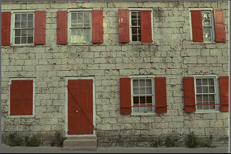
\includegraphics[width=1\textwidth]{24images/resize_kodim01.png}
\end{minipage}
\begin{minipage}{0.075\textwidth}
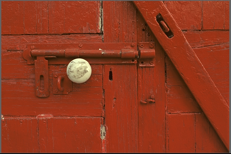
\includegraphics[width=1\textwidth]{24images/resize_kodim02.png}
\end{minipage}
\begin{minipage}{0.075\textwidth}
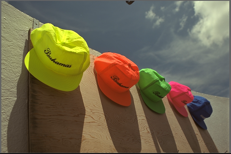
\includegraphics[width=1\textwidth]{24images/resize_kodim03.png}
\end{minipage}
\begin{minipage}{0.075\textwidth}
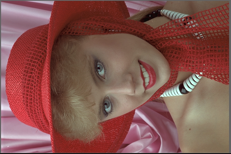
\includegraphics[width=1\textwidth]{24images/resize_kodim04.png}
\end{minipage}
\begin{minipage}{0.075\textwidth}
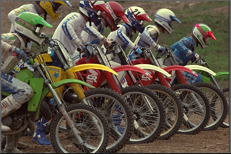
\includegraphics[width=1\textwidth]{24images/resize_kodim05.png}
\end{minipage}
\begin{minipage}{0.075\textwidth}
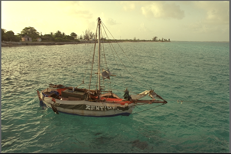
\includegraphics[width=1\textwidth]{24images/resize_kodim06.png}
\end{minipage}
}\vspace{-3mm}
\subfigure{
\begin{minipage}{0.075\textwidth}
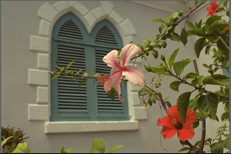
\includegraphics[width=1\textwidth]{24images/resize_kodim07.png}
\end{minipage}
\begin{minipage}{0.075\textwidth}
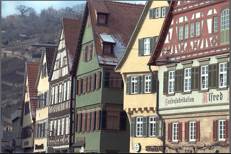
\includegraphics[width=1\textwidth]{24images/resize_kodim08.png}
\end{minipage}
\begin{minipage}{0.075\textwidth}
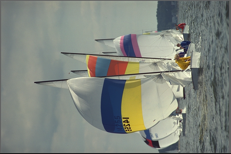
\includegraphics[width=1\textwidth]{24images/resize_kodim09.png}
\end{minipage}
\begin{minipage}{0.075\textwidth}
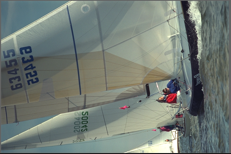
\includegraphics[width=1\textwidth]{24images/resize_kodim10.png}
\end{minipage}
\begin{minipage}{0.075\textwidth}
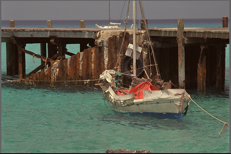
\includegraphics[width=1\textwidth]{24images/resize_kodim11.png}
\end{minipage}
\begin{minipage}{0.075\textwidth}
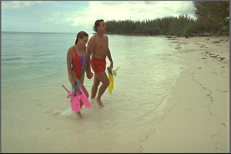
\includegraphics[width=1\textwidth]{24images/resize_kodim12.png}
\end{minipage}
}\vspace{-3mm}
\subfigure{
\begin{minipage}{0.075\textwidth}
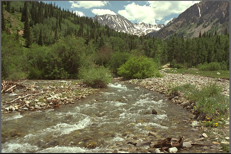
\includegraphics[width=1\textwidth]{24images/resize_kodim13.png}
\end{minipage}
\begin{minipage}{0.075\textwidth}
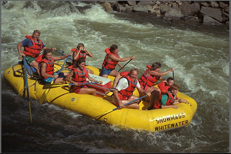
\includegraphics[width=1\textwidth]{24images/resize_kodim14.png}
\end{minipage}
\begin{minipage}{0.075\textwidth}
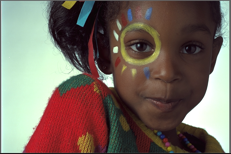
\includegraphics[width=1\textwidth]{24images/resize_kodim15.png}
\end{minipage}
\begin{minipage}{0.075\textwidth}
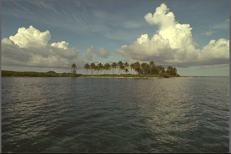
\includegraphics[width=1\textwidth]{24images/resize_kodim16.png}
\end{minipage}
\begin{minipage}{0.075\textwidth}
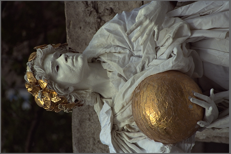
\includegraphics[width=1\textwidth]{24images/resize_kodim17.png}
\end{minipage}
\begin{minipage}{0.075\textwidth}
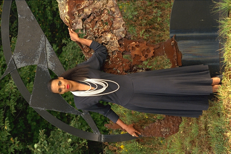
\includegraphics[width=1\textwidth]{24images/resize_kodim18.png}
\end{minipage}
}\vspace{-3mm}
\subfigure{
\begin{minipage}{0.075\textwidth}
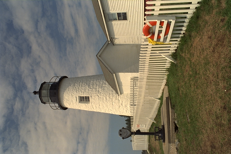
\includegraphics[width=1\textwidth]{24images/resize_kodim19.png}
\end{minipage}
\begin{minipage}{0.075\textwidth}
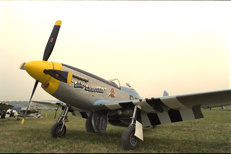
\includegraphics[width=1\textwidth]{24images/resize_kodim20.png}
\end{minipage}
\begin{minipage}{0.075\textwidth}
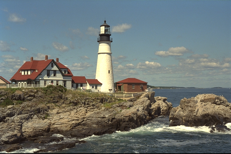
\includegraphics[width=1\textwidth]{24images/resize_kodim21.png}
\end{minipage}
\begin{minipage}{0.075\textwidth}
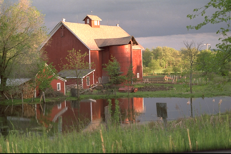
\includegraphics[width=1\textwidth]{24images/resize_kodim22.png}
\end{minipage}
\begin{minipage}{0.075\textwidth}
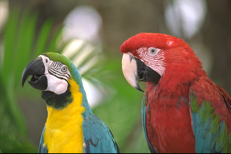
\includegraphics[width=1\textwidth]{24images/resize_kodim23.png}
\end{minipage}
\begin{minipage}{0.075\textwidth}
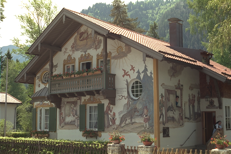
\includegraphics[width=1\textwidth]{24images/resize_kodim24.png}
\end{minipage}
}\vspace{-1mm}
\caption{The 24 high quality color images from the Kodak PhotoCD Dataset.}
\label{fig3}
\vspace{-2mm}
\end{figure}


\begin{table*}
\caption{PSNR(dB) results of different denoising algorithms on 20 natural images.}
\label{taba}
\begin{center}
\renewcommand\arraystretch{1.0}
\scriptsize
\begin{tabular}{|c||c|c|c|c|c|c|c|c|c|}
\hline
&\multicolumn{9}{c|}{ $\sigma_{r} = 40, \sigma_{g} = 20, \sigma_{b} = 30$}
\\
\hline
\hline
Image\#
&
\textbf{CBM3D}
&
\textbf{MLP}
&
\textbf{TNRD}
&
\textbf{Noise Clinic}
&
\textbf{Neat Image}
&
\textbf{WNNM}
&
\textbf{WNNM1}
&
\textbf{WNNM2}
&
\textbf{Proposed}
\\
\hline
1& 25.24 & 25.70 & 25.74 & 24.90 & 23.85 & 26.01 & 25.95 &  & 26.66
\\
\hline
2& 28.27 & 30.12 & 30.21 & 25.87 & 25.90 & 30.08 & 30.11 &  & 30.20 
\\
\hline
3 & 28.81 & 31.19 & 31.49 & 28.58 & 26.00 & 31.58 & 31.61 &  & 32.25  
\\
\hline 
4 & 27.95 & 29.88 & 29.86 & 25.67 & 25.82 & 30.13 & 30.16 &  & 30.49 
\\
\hline
5 & 25.03 & 26.00 & 26.18 & 25.15 & 24.38 & 26.44 & 26.39 &  & 26.82
\\
\hline
6 & 26.24 & 26.84 & 26.90 & 24.74 & 24.65 & 27.39 & 27.30 &  & 27.98 
\\
\hline
7 & 27.88 & 30.28 & 30.40 & 27.69 & 25.63 & 30.47 & 30.54 &  & 30.98 
\\
\hline
8 & 25.05 & 25.59 & 25.83 & 25.30 & 24.02 & 26.71 & 26.75 &  & 26.90
\\
\hline
9 & 28.44 & 30.75 & 30.81 & 27.44 & 25.94 & 30.86 & 30.92 &  & 31.49
\\
\hline
10 & 28.27 & 30.38 & 30.57 & 28.42 & 25.87 & 30.65 & 30.68 &  & 31.26
\\
\hline
11 & 26.95 & 28.00 & 28.14 & 24.67 & 25.32 & 28.19 & 28.16 &  & 28.63
\\
\hline
12 & 28.76 & 30.87 & 31.05 & 28.37 & 26.01 & 30.97 & 31.06 &  & 31.48
\\
\hline
13 & 23.76 & 23.95 & 23.99 & 22.76 & 23.53 & 24.27 & 24.15 &  & 24.89
\\
\hline
14 & 26.02 & 26.97 & 27.11 & 25.68 & 24.94 & 27.20 & 27.15 &  & 27.57
\\
\hline
15 & 28.38 & 30.15 & 30.44 & 28.21 & 26.06 & 30.52 & 30.60 &  & 30.81
\\
\hline
16 & 27.75 & 28.82 & 28.87 & 26.66 & 25.69 & 29.27 & 29.21 &  & 29.96
\\
\hline
17 & 27.90 & 29.57 & 29.80 & 28.32 & 25.85 & 29.78 & 29.79 &  & 30.40
\\
\hline
18 & 25.77 & 26.40 & 26.41 & 25.70 & 24.74 & 26.63 & 26.56 &  & 27.22
\\
\hline
19 & 27.30 & 28.67 & 28.81 & 26.52 & 25.40 & 29.19 & 29.22 &  & 29.57 
\\
\hline
20 & 28.96 & 30.40 & 30.76 & 25.90 & 24.95 & 30.79 & 30.83 &  & 31.07
\\
\hline
21 & 26.54 & 27.53 & 27.60 & 26.48 & 25.06 & 27.80 & 27.75 &  & 28.34
\\
\hline
22 & 27.05 & 28.17 & 28.27 & 26.60 & 25.36 & 28.21 & 28.16 &  & 28.64
\\
\hline
23 & 29.14 & 32.31 & 32.51 & 23.24 & 26.13 & 31.89 & 31.97 &  & 32.34
\\
\hline
24 & 25.75 & 26.41 & 26.53 & 25.73 & 24.55 & 27.10 & 27.03 &  & 27.59
\\
\hline
\textbf{Average} & 27.13 & 28.54 & 28.68 & 26.19 & 25.24 & 28.84 & 28.83 &  & 29.31
\\
\hline
\end{tabular}
\end{center}
\end{table*}

\begin{figure*}\vspace{1mm}
\centering
\subfigure{
\begin{minipage}[t]{0.195\textwidth}
\centering
\raisebox{-0.15cm}{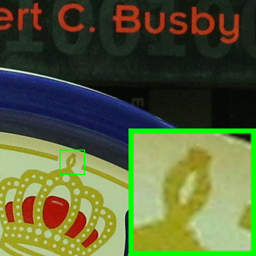
\includegraphics[width=1\textwidth]{images/resize_br_Noisy_5dmark3_iso3200_1_real.png}}
{\footnotesize (a) Noisy  \cite{crosschannel2016}: 37.00dB }
\end{minipage}
\begin{minipage}[t]{0.195\textwidth}
\centering
\raisebox{-0.15cm}{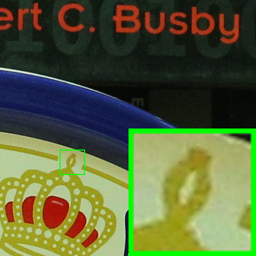
\includegraphics[width=1\textwidth]{images/resize_br_CBM3D_5dmark3_iso3200_1_real.png}}
{\footnotesize (b) CBM3D \cite{bm3d,cbm3d}: 37.02dB}
\end{minipage}
\begin{minipage}[t]{0.195\textwidth}
\centering
\raisebox{-0.15cm}{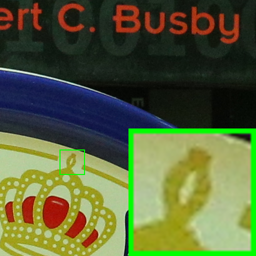
\includegraphics[width=1\textwidth]{images/resize_br_WNNM_5dmark3_iso3200_1_real.png}}
{\footnotesize (c) WNNM \cite{wnnm}: 37.01dB}
\end{minipage}
\begin{minipage}[t]{0.195\textwidth}
\centering
\raisebox{-0.15cm}{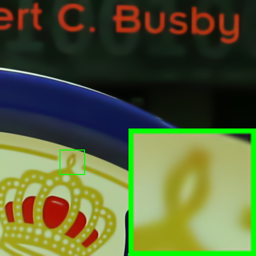
\includegraphics[width=1\textwidth]{images/resize_br_MLP_5dmark3_iso3200_1_real.png}}
{\footnotesize (d) MLP \cite{mlp}: 33.90dB }
\end{minipage}
\centering
\begin{minipage}[t]{0.195\textwidth}
\raisebox{-0.15cm}{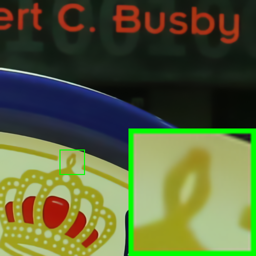
\includegraphics[width=1\textwidth]{images/resize_br_TRD_5dmark3_iso3200_1_real.png}}
{\footnotesize (e) TNRD \cite{chen2015learning}: 36.18dB  } 
\end{minipage}
}\vspace{-3mm}
\subfigure{
\begin{minipage}[t]{0.195\textwidth}
\centering
\raisebox{-0.15cm}{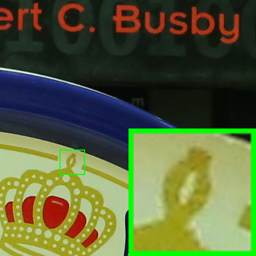
\includegraphics[width=1\textwidth]{images/resize_br_NI_5dmark3_iso3200_1_real.png}}
{\footnotesize (f) NI \cite{neatimage}: 37.68dB  }
\end{minipage}
\begin{minipage}[t]{0.195\textwidth}
\centering
\raisebox{-0.15cm}{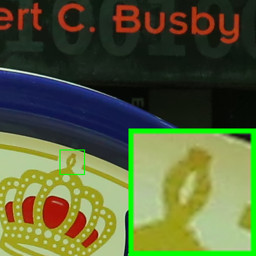
\includegraphics[width=1\textwidth]{images/resize_br_NC_5dmark3_iso3200_1_real.png}}
{\footnotesize (g) NC \cite{noiseclinic,ncwebsite}: 38.76dB  }
\end{minipage}
\begin{minipage}[t]{0.195\textwidth}
\centering
\raisebox{-0.15cm}{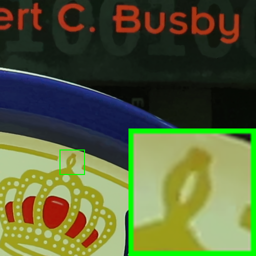
\includegraphics[width=1\textwidth]{images/resize_br_CCNoise_5dmark3_iso3200_1.png}}
{\footnotesize (h) CC \cite{crosschannel2016}: 38.37dB }
\end{minipage}
\begin{minipage}[t]{0.195\textwidth}
\centering
\raisebox{-0.15cm}{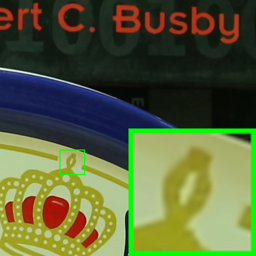
\includegraphics[width=1\textwidth]{images/resize_br_Guided_5dmark3_iso3200_1_real.png}}
{\footnotesize (i) Ours: \textbf{40.50}dB}
\end{minipage}
\begin{minipage}[t]{0.195\textwidth}
\centering
\raisebox{-0.15cm}{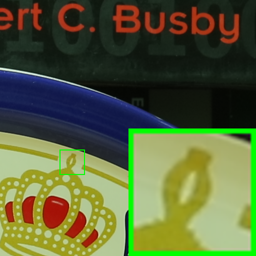
\includegraphics[width=1\textwidth]{images/resize_br_Mean_5dmark3_iso3200_1_real.png}}
{\footnotesize (j) Mean Image \cite{crosschannel2016}}
\end{minipage}
}\vspace{-0.5mm}
\caption{Denoised images of a region cropped from the real noisy image ``Canon 5D Mark 3 ISO 3200 1" \cite{crosschannel2016} by different methods. The images are better to be zoomed in on screen.}
\label{fig7}
\vspace{0.5mm}
\end{figure*}

\subsection{Experiments on Real Noisy Images}
In the second part, we compare the proposed method with other competing methods on the 15 real noisy images, , which are shown in Fig.\ 2, with ``ground truth'' clean images \cite{crosschannel2016}. The noisy images were collected under controlled indoor environment.\ Each scene was shot 500 times under the same camera and camera setting.\ The mean image of the 500 shots is roughly taken as the ``ground truth", with which the PSNR can be computed. Since the image size is very large (about $7000\times5000$) and the scenes of this dataset share repetitive contents, the authors of \cite{crosschannel2016} cropped 15 smaller images (of size $512\times512$) to perform experiments. In this section, we do not compare with the ``WNNMCW'' method due to its inferior performance.

We firstly perform quantitative comparison on the 15 cropped images used in \cite{crosschannel2016}. The PSNR results of CBM3D \cite{bm3d}, WNNM \cite{wnnm}, MLP \cite{mlp}, TNRD \cite{chen2015learning}, NC \cite{noiseclinic,ncwebsite}, NI \cite{neatimage} and
CC \cite{crosschannel2016} are listed in Table \ref{tabb} (The results of CC are copied from the original paper \cite{crosschannel2016}).\ The best and second best PSNR results of each image are highlighted in red and blue, respectively.\ One can see that on 9 out of the 15 images, our method achieves the best PSNR values.\ CC achieves the best PSNR on 3 of the 15 images.\ It should be noted that in the CC method, a specific model is trained for each camera and camera setting, while our method uses the same model for all images.\ On average, our proposed method has 0.28dB PSNR improvements over \cite{crosschannel2016} and much higher PSNR gains over other competing methods.\ Fig.\ \ref{fig7} shows the denoised images of a scene captured by Canon 5D Mark 3 at ISO = 3200.\ We can see that CBM3D, WNNM, NC, NI and CC would either remain noise or generate artifacts, while MLP, TNRD over-smooth much the image.\ By using the proposed multi-channel WNNM model, our method preserves the structures (e.g., edges and textures) better across the R, G, B channels and generate less artifacts than other denoising methods, leading to visually pleasant outputs.\ More visual comparisons can be found in the supplementary file.

\begin{figure}
\centering
\subfigure{
\begin{minipage}{0.085\textwidth}
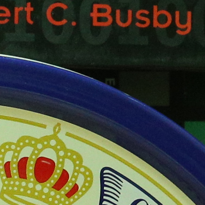
\includegraphics[width=1\textwidth]{CC15images/resize_5dmark3_iso3200_1_real.png}
\end{minipage}
\begin{minipage}{0.085\textwidth}
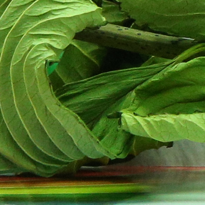
\includegraphics[width=1\textwidth]{CC15images/resize_5dmark3_iso3200_2_real.png}
\end{minipage}
\begin{minipage}{0.085\textwidth}
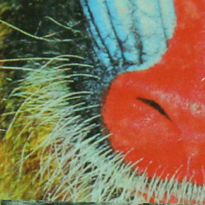
\includegraphics[width=1\textwidth]{CC15images/resize_5dmark3_iso3200_3_real.png}
\end{minipage}
\begin{minipage}{0.085\textwidth}
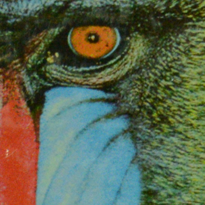
\includegraphics[width=1\textwidth]{CC15images/resize_d600_iso3200_1_real.png}
\end{minipage}
\begin{minipage}{0.085\textwidth}
\includegraphics[width=1\textwidth]{CC15images/resize_d600_iso3200_2_real.png}
\end{minipage}
}\vspace{-3mm}
\subfigure{
\begin{minipage}{0.085\textwidth}
\includegraphics[width=1\textwidth]{CC15images/resize_d600_iso3200_3_real.png}
\end{minipage}
\begin{minipage}{0.085\textwidth}
\includegraphics[width=1\textwidth]{CC15images/resize_d800_iso1600_1_real.png}
\end{minipage}
\begin{minipage}{0.085\textwidth}
\includegraphics[width=1\textwidth]{CC15images/resize_d800_iso1600_2_real.png}
\end{minipage}
\begin{minipage}{0.085\textwidth}
\includegraphics[width=1\textwidth]{CC15images/resize_d800_iso1600_3_real.png}
\end{minipage}
\begin{minipage}{0.085\textwidth}
\includegraphics[width=1\textwidth]{CC15images/resize_d800_iso3200_1_real.png}
\end{minipage}
}\vspace{-3mm}
\subfigure{
\begin{minipage}{0.085\textwidth}
\includegraphics[width=1\textwidth]{CC15images/resize_d800_iso3200_2_real.png}
\end{minipage}
\begin{minipage}{0.085\textwidth}
\includegraphics[width=1\textwidth]{CC15images/resize_d800_iso3200_3_real.png}
\end{minipage}
\begin{minipage}{0.085\textwidth}
\includegraphics[width=1\textwidth]{CC15images/resize_d800_iso6400_1_real.png}
\end{minipage}
\begin{minipage}{0.085\textwidth}
\includegraphics[width=1\textwidth]{CC15images/resize_d800_iso6400_2_real.png}
\end{minipage}
\begin{minipage}{0.085\textwidth}
\includegraphics[width=1\textwidth]{CC15images/resize_d800_iso6400_3_real.png}
\end{minipage}
}\vspace{-1mm}
\caption{The 15 cropped real noisy images used in \cite{crosschannel2016}.}
\label{fig3}
\vspace{-2mm}
\end{figure}


\begin{table*}\vspace{2mm}
\caption{PSNR(dB) results of different methods on 15 cropped real noisy images used in \cite{crosschannel2016}.}
\vspace{0.5mm}
\label{tabb}
\begin{center}
\renewcommand\arraystretch{1}
\begin{tabular}{|c||c|c|c|c|c|c|c|c|c|}
\hline
Camera Settings  
&
\textbf{CBM3D}
&
\textbf{MLP}
&
\textbf{TNRD}
&
\textbf{NI}
&
\textbf{NC}
&
\textbf{CC}
&
\textbf{WNNM1}
&
\textbf{WNNM2}
&
\textbf{Proposed} 
\\
\hline
\multirow{3}{*}{\small{Canon 5D Mark III}}  
& 39.76 & 39.00 & 39.51 & 35.68 & 36.20 & 38.37 & 39.74 & 39.98 & \textbf{41.13}
\\ 
\cdashline{2-10} 
\multirow{3}{*}{ISO = 3200}   
 & 36.40 & 36.34 & 36.47 & 34.03 & 34.35 & 35.37 & 35.12 & 36.65 & \textbf{37.28}
\\ 
\cdashline{2-10}    
 & 36.37 & 36.33 & 36.45 & 32.63 & 33.10& 34.91 & 33.14 & 34.63 & \textbf{36.52}  
\\
\hline
\multirow{3}{*}{Nikon D600} 
 & 34.18 & 34.70 & 34.79 & 31.78 & 32.28 & 34.98 & 35.08 & 35.08 & \textbf{35.53}
\\ 
\cdashline{2-10} 
\multirow{3}{*}{ISO = 3200}   
 & 35.07 & 36.20 & 36.37 & 35.16 & 35.34 & 35.95 & 36.42 & 36.84 & \textbf{37.02}
\\ 
\cdashline{2-10}    
 & 37.13 & 39.33 & 39.49 & 39.98 & 40.51 & \textbf{41.15} & 40.78 & 39.24 & 39.56
\\
\hline
\multirow{3}{*}{Nikon D800} 
 & 36.81  & 37.95 & 38.11 & 34.84 & 35.09 & 37.99 & 38.28 & 38.61 & \textbf{39.26}
\\ 
\cdashline{2-10} 
\multirow{3}{*}{ISO = 1600}   
 & 37.76 & 40.23 & 40.52 & 38.42 & 38.65 & 40.36 & 41.24 & 40.81 & \textbf{41.43}
\\ 
\cdashline{2-10}    
 & 37.51 & 37.94 & 38.17 & 35.79 & 35.85 & 38.30 & 38.04 & 38.96 & \textbf{39.55}
\\
\hline
\multirow{3}{*}{Nikon D800} 
 & 35.05 & 37.55 & 37.69 & 38.36 & 38.56 & \textbf{39.01} & 39.93 & 37.97 & 38.91
\\ 
\cdashline{2-10} 
\multirow{3}{*}{ISO = 3200}   
 & 34.07 & 35.91 & 35.90 & 35.53 & 35.76 & 36.75 & 37.32 & 37.30 & \textbf{37.41}
\\ 
\cdashline{2-10}    
 & 34.42 & 38.15 & 38.21 & 40.05 & 40.59 & 39.06 & \textbf{41.52} & 38.68 & 39.39
\\ 
\hline
\multirow{3}{*}{Nikon D800} 
& 31.13 & 32.69 & 32.81 & 34.08 & 34.25 & 34.61 & \textbf{35.20} & 34.57 & 34.80
\\ 
\cdashline{2-10} 
\multirow{3}{*}{ISO = 6400}   
 & 31.22 & 32.33 & 32.33 & 32.13 & 32.38  & 33.21 & 33.61 & 33.43 & \textbf{33.95}
\\ 
\cdashline{2-10}    
 & 30.97 & 32.29 & 32.29 & 31.52 & 31.76 & 33.22 & 33.62 & 34.02 & \textbf{33.94}
\\
\hline
Average & 35.19 & 36.46 & 36.61 & 35.33 & 35.65 & 36.88 & 37.27 & 37.12 & \textbf{ 37.71}
\\
\hline
\end{tabular}
\end{center}
\vspace{1mm}
\end{table*}

\begin{figure*}\vspace{1mm}
\centering
\subfigure{
\begin{minipage}[t]{0.195\textwidth}
\centering
\raisebox{-0.15cm}{\includegraphics[width=1\textwidth]{images/resize_br_Noisy_5dmark3_iso3200_1_real.png}}
{\footnotesize (a) Noisy  \cite{crosschannel2016}: 37.00dB }
\end{minipage}
\begin{minipage}[t]{0.195\textwidth}
\centering
\raisebox{-0.15cm}{\includegraphics[width=1\textwidth]{images/resize_br_CBM3D_5dmark3_iso3200_1_real.png}}
{\footnotesize (b) CBM3D \cite{bm3d,cbm3d}: 37.02dB}
\end{minipage}
\begin{minipage}[t]{0.195\textwidth}
\centering
\raisebox{-0.15cm}{\includegraphics[width=1\textwidth]{images/resize_br_WNNM_5dmark3_iso3200_1_real.png}}
{\footnotesize (c) WNNM \cite{wnnm}: 37.01dB}
\end{minipage}
\begin{minipage}[t]{0.195\textwidth}
\centering
\raisebox{-0.15cm}{\includegraphics[width=1\textwidth]{images/resize_br_MLP_5dmark3_iso3200_1_real.png}}
{\footnotesize (d) MLP \cite{mlp}: 33.90dB }
\end{minipage}
\centering
\begin{minipage}[t]{0.195\textwidth}
\raisebox{-0.15cm}{\includegraphics[width=1\textwidth]{images/resize_br_TRD_5dmark3_iso3200_1_real.png}}
{\footnotesize (e) TNRD \cite{chen2015learning}: 36.18dB  } 
\end{minipage}
}\vspace{-3mm}
\subfigure{
\begin{minipage}[t]{0.195\textwidth}
\centering
\raisebox{-0.15cm}{\includegraphics[width=1\textwidth]{images/resize_br_NI_5dmark3_iso3200_1_real.png}}
{\footnotesize (f) NI \cite{neatimage}: 37.68dB  }
\end{minipage}
\begin{minipage}[t]{0.195\textwidth}
\centering
\raisebox{-0.15cm}{\includegraphics[width=1\textwidth]{images/resize_br_NC_5dmark3_iso3200_1_real.png}}
{\footnotesize (g) NC \cite{noiseclinic,ncwebsite}: 38.76dB  }
\end{minipage}
\begin{minipage}[t]{0.195\textwidth}
\centering
\raisebox{-0.15cm}{\includegraphics[width=1\textwidth]{images/resize_br_CCNoise_5dmark3_iso3200_1.png}}
{\footnotesize (h) CC \cite{crosschannel2016}: 38.37dB }
\end{minipage}
\begin{minipage}[t]{0.195\textwidth}
\centering
\raisebox{-0.15cm}{\includegraphics[width=1\textwidth]{images/resize_br_Guided_5dmark3_iso3200_1_real.png}}
{\footnotesize (i) Ours: \textbf{40.50}dB}
\end{minipage}
\begin{minipage}[t]{0.195\textwidth}
\centering
\raisebox{-0.15cm}{\includegraphics[width=1\textwidth]{images/resize_br_Mean_5dmark3_iso3200_1_real.png}}
{\footnotesize (j) Mean Image \cite{crosschannel2016}}
\end{minipage}
}\vspace{-0.5mm}
\caption{Denoised images of a region cropped from the real noisy image ``Canon 5D Mark 3 ISO 3200 1" \cite{crosschannel2016} by different methods. The images are better to be zoomed in on screen.}
\label{fig7}
\vspace{0.5mm}
\end{figure*}

\section{Conclusion and Future Work}
Most existing color image denoising methods treat the R, G, B channels equally and ignore the different noise structures in different channels. Common strategies that processing each channel seperately and concatenating the RGB values into joint vectors would generate false color or artifacts. In this paper, we proposed a noval model for color image denoising which can explore the different noise structures among the R, G, B channels and exploit the non-local self similarity property of natural images. Specifically, we introduced a weighting matrix, which are employed to describe the noise levels of different channels, to the original weighted nuclear norm minimization (WNNM) model. Though the proposed model no longer has closed-form solution, we successfully solved the proposed model via the famous ADMM algorithm by introducing an additional variable with a linear constraint. The transformed problem has convergence property and can be solved in an alternative updating manner and both variables can be updated with closed-form solutions. We applied the proposed multi-channel WNNM model on color image denoising problem. Extensive experiments on benchmark datasets demonstrate that the proposed model outperforms the other competing denoising methods on both synthetic color noisy images as well as real-world noisy images. The introduce of the weighting matrix can indeed boost the performance of the original WNNM model on color image denoising. We believe that this work can be extended in at least three directions. Firstly, the proposed weighting matrix can be introduced into other methods designed for denoising grayscale images. Secondly, the weighting matrix beyond the diagonal form, such as correlation form \cite{nearcor}, may bring better performance on color image denoising. Thirdly, the proposed multi-channel WNNM model can be further extended to deal with images with more channels, such as the hyperspectral images in remote sensing applications. We will focus our futhre work on these three directions.



{
\small
\bibliographystyle{unsrt}
\bibliography{egbib}
}

\end{document}